%======================================================================
\chapter{An Example of Converting a Boolean Circuit to R1CS}\label{a_ch:r1cs_from_circuit}
%======================================================================


In this appendix we adopt an example from \cite{Gong2024} which shows the computation of rank-1 constraint system (\gls{r1cs}) instance from encoding a Boolean circuit depicted in Figure \ref{fig:Arith-circuit}. To encode the circuit to an \gls{r1cs} instance, we are going to find $\mathbf{A}, \mathbf{B}, \mathbf{C} \in \mathbb{F}_2^{{d_1}\times{(d_2+1)}}$ matrices for the circuit, where $d_1 = 3$ denotes the number of  \texttt{AND} gates (number of constraints) and $d_2 = 7$ denotes the number of variables. We have three \texttt{AND} gates, denoted as $\text{\textbf{gate}}_i$. Let vector $\vec{z}^\intercal=(z_0, z_1, \ldots, z_7)$ where $z_0=1$ represents inputs and wire values, Table \ref{tab:gates} shows left and right inputs and output of each gate.

\begin{figure}[h]
	\centering
	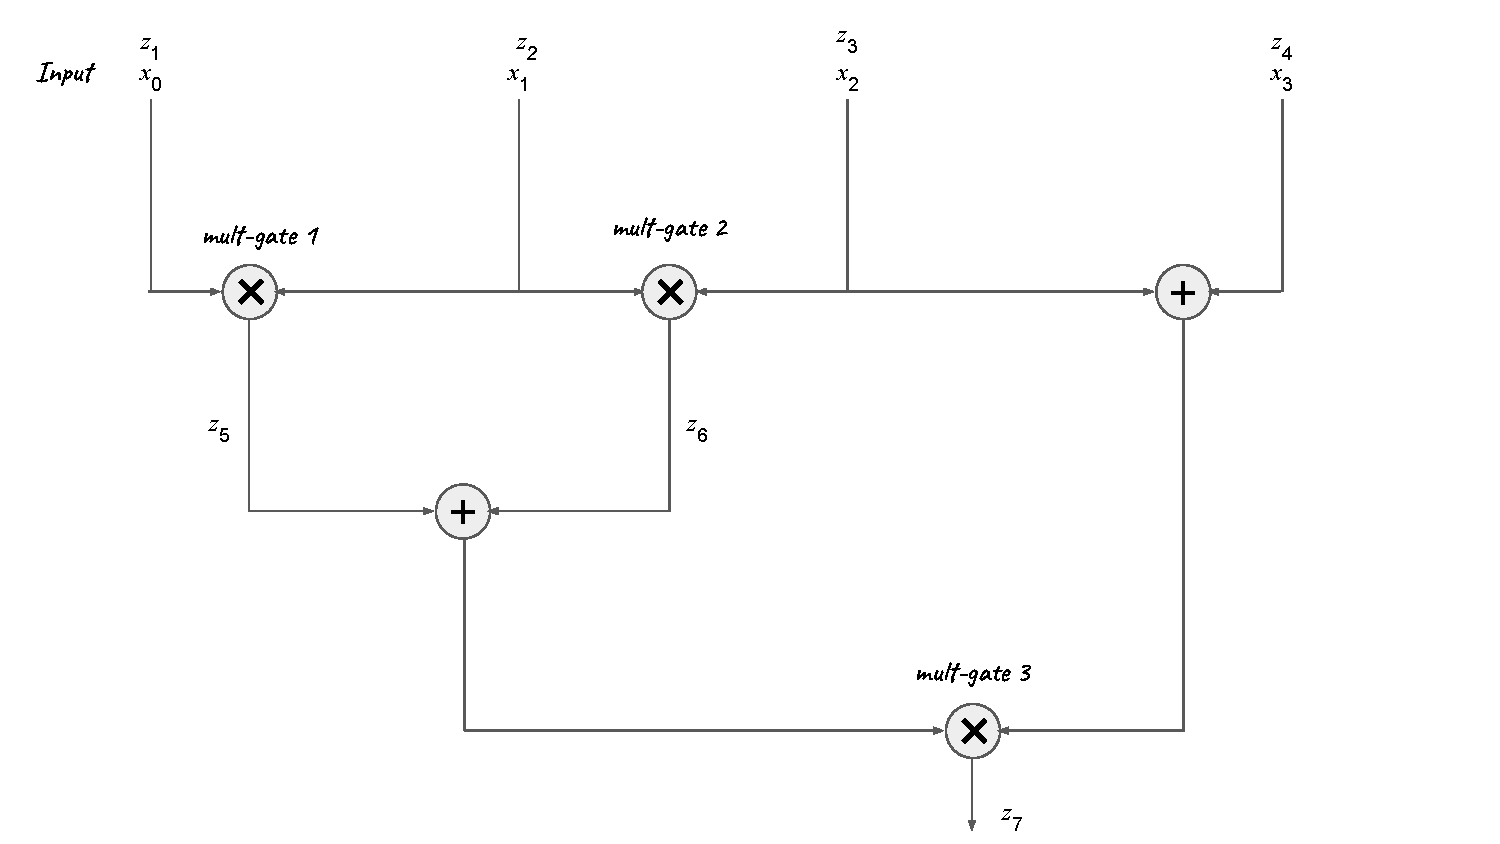
\includegraphics[width=\textwidth]{Figures/Circuit.pdf}
	\caption[An example of a Boolean circuit]{An example of a Boolean circuit in which \textit{mult-gates} are  \texttt{AND} gates.}
	\label{fig:Arith-circuit}
\end{figure}




\begin{table}[h]
	\centering
\caption[Left and right inputs and output of gates in the example circuit]{Left and right inputs, along with the output of each gate. \texttt{XOR} gates are merged into \texttt{AND} gates.}

	\begin{tabular}{c c c c c c c}
		\toprule
		\textbf{$\text{gate}_i$} & $g_l$& & $g_r$& & $g_o$ &  \\
		\midrule
		1 & $z_1$& $\wedge$ & $z_2$& $\oplus$ & $z_5$ & $= 0$\\

		2 & $z_2$& $\wedge$ & $z_3$& $\oplus$ & $z_6$ & $= 0$\\

		3 & $(z_5 \oplus z_6)$& $\wedge$ & $( z_3 \oplus z_4)$& $\oplus$ & $z_7$ & $= 0$\\
		\bottomrule
	\end{tabular}
	\label{tab:gates}
\end{table}

Accordingly, we can make $\mathbf{A}, \mathbf{B}, \mathbf{C}$ matrices:
\begin{equation}
	\label{eq:ABC-example}
	A = 
	\begin{bmatrix}
		0 & 1 & 0 & 0 & 0 & 0 & 0 & 0\\
		0 & 0 & 1 & 0 & 0 & 0 & 0 & 0\\
		0 & 0 & 0 & 0 & 0 & 1 & 1 & 0
	\end{bmatrix}, B = 
	\begin{bmatrix}
		0 & 0 & 1 & 0 & 0 & 0 & 0 & 0\\
		0 & 0 & 0 & 1 & 0 & 0 & 0 & 0\\
		0 & 0 & 0 & 1 & 1 & 0 & 0 & 0
	\end{bmatrix},
	 C = 
	\begin{bmatrix}
		0 & 0 & 0 & 0 & 0 & 1 & 0 & 0\\
		0 & 0 & 0 & 0 & 0 & 0 & 1 & 0\\
		0 & 0 & 0 & 0 & 0 & 0 & 0 & 1
	\end{bmatrix}
\end{equation}

Consequently, setting $(z_1, z_2, z_3, z_4) = (1, 1, 0, 1)$ (inputs) results the remaining $(z_5, z_6, z_7) = (1, 0, 1)$ which are internal wires or the output. Hence, $\vec{z}^\intercal=(1, 1, 1, 0, 1, 1, 0, 1)$. The computed $\vec{z}$ satisfies $(A\cdot \vec{z})\circ(B\cdot \vec{z})-(C\cdot \vec{z})=0$.
